In this chapter, I present the implementation of a two-qubit destructive SWAP test, introduced by García-Escartín et al.~\cite{Garcia_Escartin_2013}. Unlike the conventional SWAP test, this protocol does not require an ancillary qubit, at the cost of requiring the measurement of the target quantum states. I also show how the scalar product between the two quantum states can be extracted from the measurement outcomes of the destructive SWAP test. Finally, I describe the design and successive optimization of a control pulse sequence that implements this operation on the \acs{nmr} quantum computer used in this work.

\section{The SWAP test}
\label{sec:swaptest}

A conventional SWAP test requires three qubits, one of which serves as an ancillary qubit. The circuit begins with a Hadamard gate applied to the ancilla, followed by a controlled-SWAP (Fredkin) gate acting on the two target qubits and controlled by the state of the ancilla. A second Hadamard gate is then applied to the ancillary qubit before measurement.

\begin{figure}[h]
\centering
\scalebox{1.3}{
\Qcircuit@C=1.0em @R=0.3em @!R { \\
                \nghost{{q}_{0}:  } & \lstick{{q}_{0}:  } & \gate{\mathrm{H}} & \ctrl{1} & \gate{\mathrm{H}} & \meter& \qw\\
                \nghost{{q}_{1}:  } & \lstick{{q}_{1}:  } & \qw& \qswap& \qw& \qw& \qw\\
                \nghost{{q}_{2}:  } & \lstick{{q}_{2}:  } & \qw& \qswap\qwx[-1] & \qw& \qw& \qw\\
\\ }}
\caption{Conventional SWAP test}
\end{figure}


\begin{equation}
\begin{aligned}
    |0\rangle |\psi\rangle |\phi\rangle &\xrightarrow{\mathrm{Hadamard}}\frac{|0\rangle+|1\rangle}{\sqrt{2}}|\psi\rangle |\phi\rangle\\&\xrightarrow{\mathrm{CSWAP}}\frac{|0\rangle|\psi\rangle|\phi\rangle+|1\rangle|\phi\rangle|\psi\rangle}{\sqrt{2}}\\&\xrightarrow{\mathrm{Hadamard}}\frac{|0\rangle[|\psi\rangle|\phi\rangle+|\phi\rangle|\psi\rangle]+|1\rangle[|\psi\rangle|\phi\rangle-|\phi\rangle|\psi\rangle]}{2}
\end{aligned}
\end{equation}

If the two quantum states are identical, measuring the ancillary qubit always yields the state \(|0\rangle\), since the antisymmetric component of the joint state vanishes: \(|\psi\rangle|\phi\rangle-|\phi\rangle|\psi\rangle=0\). More generally, the probability of obtaining the outcome \(|0\rangle\) is

\begin{equation}
\begin{aligned}
     P(|0\rangle)
     &=\frac{1}{4}\left\|\,|\psi\rangle|\phi\rangle+|\phi\rangle|\psi\rangle\,\right\|^2\\
     &=\frac{1+|\langle\psi|\phi\rangle|^2}{2}.
     \label{eq:swaptest_pass}
\end{aligned}
\end{equation}

Conversely, if the two states are orthogonal, then \(|\langle\psi|\phi\rangle|=0\), and the ancilla is measured in the states \(|0\rangle\) and \(|1\rangle\) with equal probability. Repeating the experiment multiple times therefore yields each outcome with probability \(1/2\).

Motivated by the Hong–Ou–Mandel effect in quantum optics, which is used to compare the states of two photons, García-Escartín et al.\ proposed in 2013 a protocol to perform a SWAP test without the need for an ancillary qubit~\cite{Garcia_Escartin_2013}. They demonstrate that this protocol is equivalent to the conventional SWAP test by decomposing it into simpler, equivalent circuits in which the ancillary qubit is removed, and the protocol is reformulated in terms of direct measurements on the two target qubits. They further show that the method can be generalized to an arbitrary number of qubits. The circuit in Figure~\ref{fig:destructive_swap} illustrates their two-qubit implementation.

\begin{figure}[h]
\centering
\scalebox{1.3}{
\Qcircuit@C=1.0em @R=0.3em @!R {
\\
\nghost{{q}_{0}:  } & \lstick{{q}_{0}:  } & \ctrl{1} & \gate{\mathrm{H}} & \meter& \qw\\
\nghost{{q}_{1}:  } & \lstick{{q}_{1}:  } & \targ& \qw& \meter& \qw\\
\\
}}
\caption{Destructive SWAP test}
~\label{fig:destructive_swap}
\end{figure}

This circuit is effectively a measurement in the Bell basis and yields the same measurement statistics as the conventional SWAP test by measuring the two target qubits. In the destructive SWAP test, the measurement outcome \(|11\rangle\) corresponds to a projection onto the antisymmetric Bell state, \(|\Psi^-\rangle\), whose amplitude is proportional to the antisymmetric component of the joint input state. Consequently, if the two input states are identical, this antisymmetric component vanishes and the probability of measuring \(|11\rangle\) is zero.

Consider the initial states \(|\psi\rangle\) and \(|\phi\rangle\):

\begin{equation}
    |\psi\rangle= a|0\rangle+b|1\rangle,
    \qquad
    |\phi\rangle =c|0\rangle+d|1\rangle.
\end{equation}

Applying the destructive SWAP test yields

\begin{equation}
\begin{aligned}
ac|00\rangle+ad|01\rangle+bc|10\rangle+bd|11\rangle
&\xrightarrow{\mathrm{CNOT}}
ac|00\rangle+ad|01\rangle+bc|11\rangle+bd|10\rangle\\
&\xrightarrow{\mathrm{Hadamard}}
\frac{1}{\sqrt{2}}\bigl[
    ac|00\rangle+ac|10\rangle+ad|01\rangle+ad|11\rangle\\
&\hspace{2cm}
    +bc|01\rangle-bc|11\rangle+bd|00\rangle-bd|10\rangle
\bigr].
\end{aligned}
\end{equation}

From this expression, the probability of measuring \(|11\rangle\) is given by

\begin{equation}
\begin{aligned}
    P(|11\rangle)
    &= \frac{|ad-bc|^2}{2} \\
    &= \frac{{(ad-bc)}{(ad-bc)}^*}{2} \\
    &= \frac{|a|^2|d|^2-adb^*c^*-bca^*d^*+|b|^2|c|^2}{2} \\
    &= \frac{1-|\langle\psi|\phi\rangle|^2}{2}.
\end{aligned}
\end{equation}

The complementary outcome to measuring the state \(|11\rangle\), corresponding to the measurement of any of the remaining three computational basis states, yields the same probability as in Eq.~\ref{eq:swaptest_pass}

\begin{equation}
\begin{aligned}
    P_{\mathrm{pass}}
    &= 1 - P(|11\rangle) \\
    &= P(|00\rangle) + P(|01\rangle) + P(|10\rangle) \\
    &= \frac{1 + |\langle \psi | \phi \rangle|^2}{2}.
\end{aligned}
\end{equation}

The equivalence between the conventional SWAP test and the destructive SWAP test is thus established. Analogously to measuring the ancilla qubit in the state \(|0\rangle\) in the conventional SWAP test, a single measurement outcome other than \(|11\rangle\) is not sufficient to determine whether the input states are identical, as the protocol relies on probabilistic measurement outcomes. Consequently, the overlap between the input states must be inferred from measurement statistics accumulated over many repetitions. In an \acs{nmr} quantum computer, however, this requirement is naturally satisfied, since measurements are performed over an ensemble of identically prepared molecules and directly yield expectation values encoded in the measured density matrix.

From these statistical results, the scalar product between the two tested states can be extracted. This is required for the evaluation of Bargmann invariants, which are defined as products of inner products between sequences of quantum states. The destructive SWAP test therefore provides direct access to the overlaps needed to experimentally determine these geometric quantities.

\section{Pulse design}
\label{sec:pulse_design}

\subsection{GRAPE optimization}
\label{subsec:grape_optimization}

Using the algorithm described in Section~\ref{GRAPE}, a search was performed for a single control pulse implementing the complete unitary operation of the destructive SWAP test. The control amplitudes were initialized to a near-zero value (0.0001\%), the time step was fixed at 4~\(\mu\)s, and the optimization included robustness against 5\% RF field amplitude variations together with a smoothness penalty of weight \(5\times10^{-3}\).

A time sweep was then carried out for pulse durations ranging from 1~ms to 5~ms. Candidate pulses were selected for experimental implementation according to three criteria: high theoretical fidelity, short pulse duration, and a physically reasonable pulse profile. The theoretical fidelity obtained as a function of pulse duration is shown in Figure~\ref{fig:grape_swaptest}.

\begin{figure}[h]
    \centering
    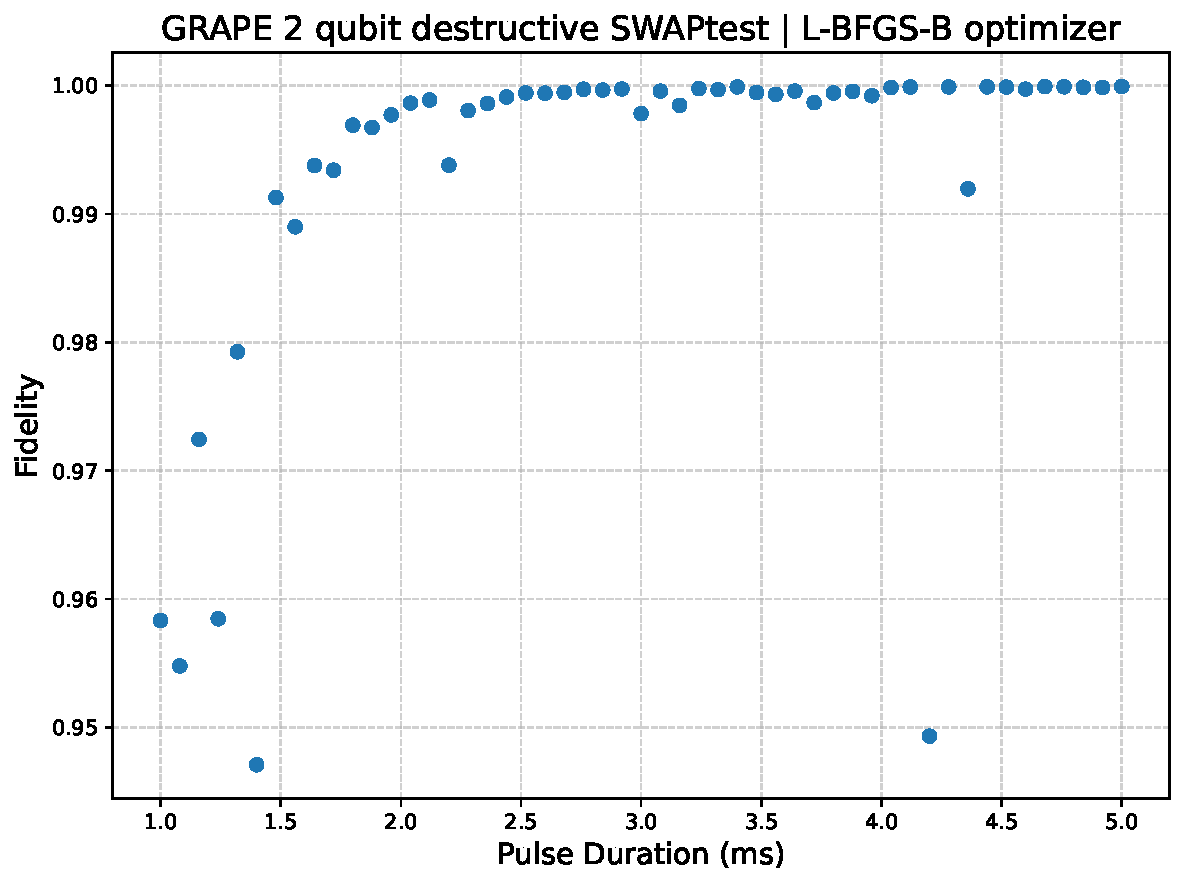
\includegraphics[width=0.8\textwidth]{images/grape_swaptest_fidelity.pdf}
    \caption{GRAPE-implemented destructive SWAP test gate theoretical fidelity for different pulse durations. Each data point represents the best theoretical fidelity obtained for a given pulse duration.}
    \label{fig:grape_swaptest}
\end{figure}

The experimental fidelity was evaluated by applying the control pulse to each of the computational basis states, \(|00\rangle\), \(|01\rangle\), \(|10\rangle\), and \(|11\rangle\). The experimentally reconstructed output state for each input was then compared with the corresponding ideal target state using the Hilbert-Schmidt inner product. The reported experimental fidelity is the average of these four state fidelities, given by

\begin{equation}
    F_{\mathrm{experimental}}
    = \frac{1}{N}\sum_{i=1}^{N}
    \mathrm{Tr}\!\left(
    \rho_{\mathrm{experimental}}^{(i)}
    \rho_{\mathrm{target}}^{(i)}
    \right),
\end{equation}

where \(N=4\) is the number of computational basis states.

The best-performing candidates, with durations of 1.8~ms and 2.12~ms, achieved theoretical fidelities exceeding 99\%. Experimentally, however, both pulses reached fidelities of only approximately 70\%, revealing a significant discrepancy between the idealized optimization model and the physical implementation. The corresponding pulse profiles are shown in Figures~\ref{fig:swap_tstudy10} and~\ref{fig:swap_tstudy14}.

\begin{figure}[h]
    \centering
    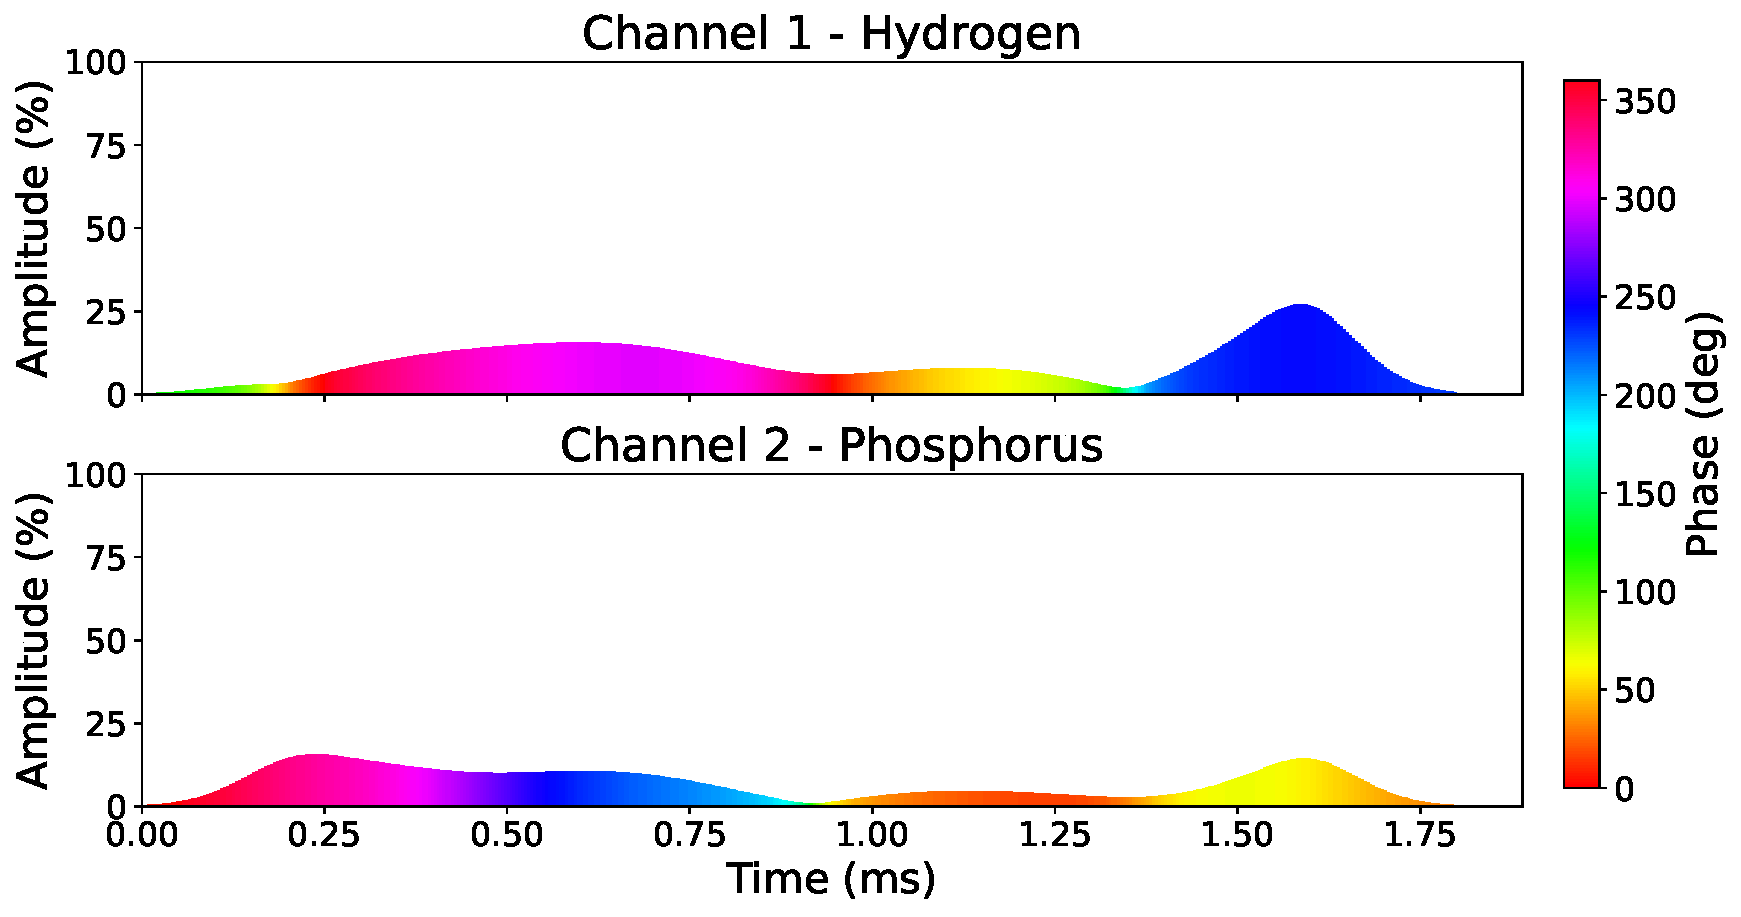
\includegraphics[width=0.8\textwidth]{images/swaptest_tstudy10.pdf}
    \caption{Pulse profile for the SWAP test optimization with a duration of 1.8~ms. Experimental fidelity of 69.2544\%.}
    \label{fig:swap_tstudy10}
\end{figure}

\begin{figure}[h]
    \centering
    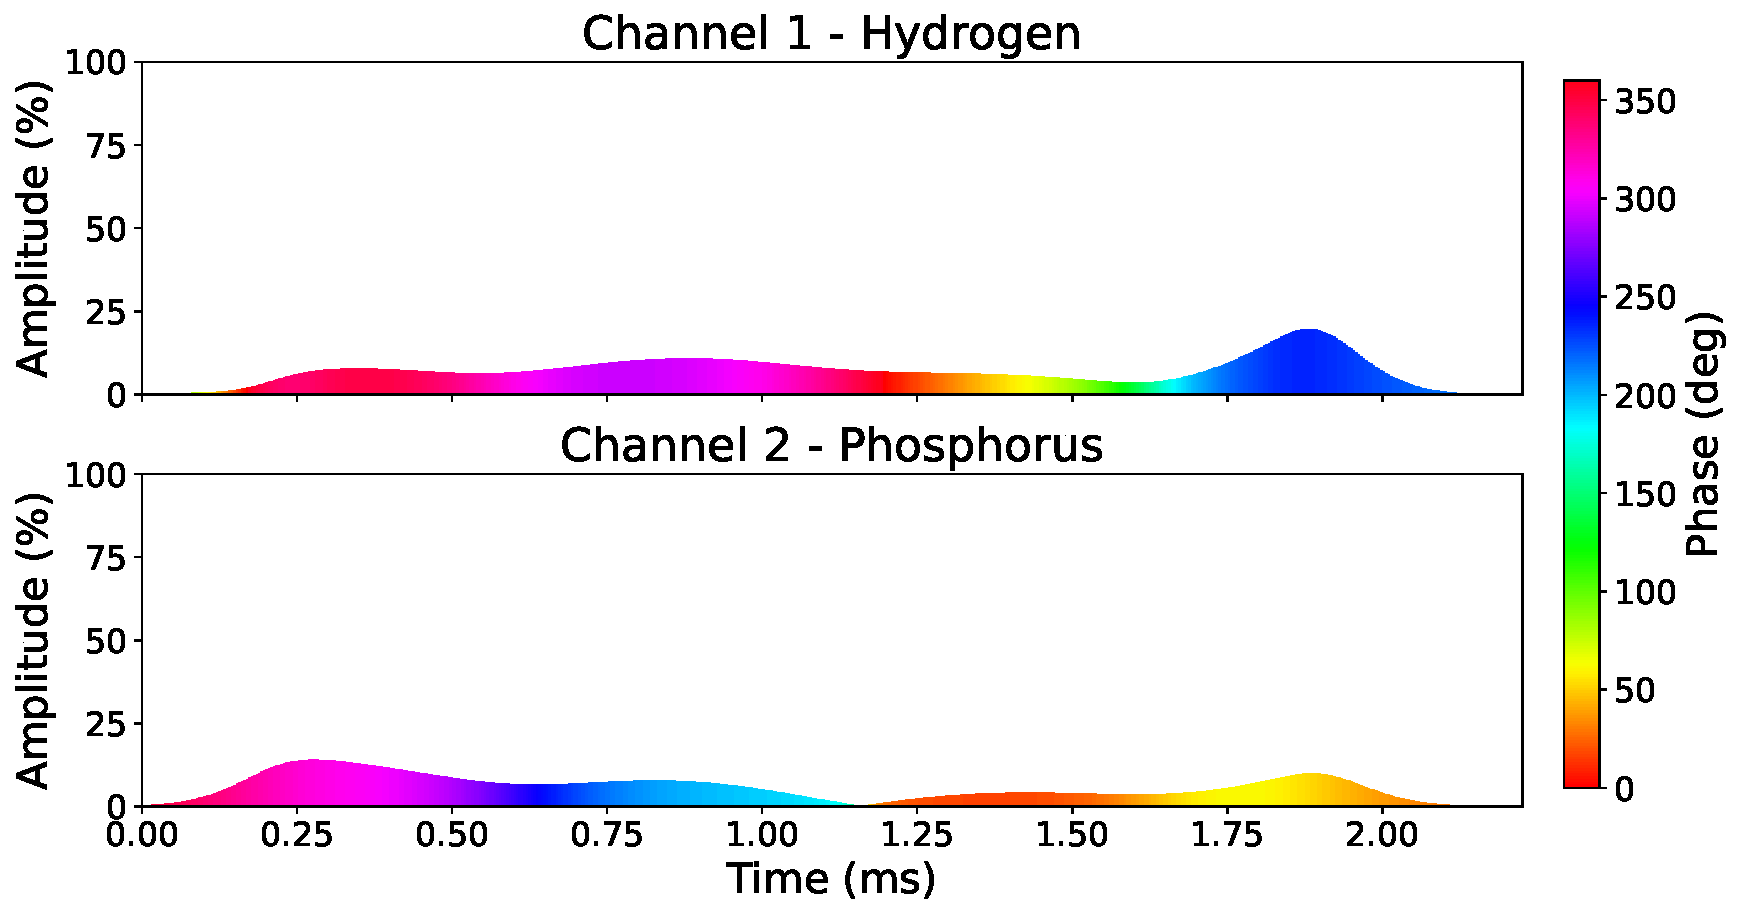
\includegraphics[width=0.8\textwidth]{images/swaptest_tstudy14.pdf}
    \caption{Pulse profile for the SWAP test optimization with a duration of 2.12~ms. Experimental fidelity of 70.1728\%.}
    \label{fig:swap_tstudy14}
\end{figure}

An experimental fidelity of around 70\% was deemed insufficient for the purpose of this work, as it would not provide a confident measurement of the overlap between the input states. 

\subsection{Composite pulse optimization}
\label{subsec:composite_pulse_optimization}

The limited experimental performance of the single-pulse optimization suggested that the optimizer was converging to suboptimal solutions. To provide a more suitable initial guess, the destructive SWAP test was broken down into its component operations and optimized separately.

A CNOT gate was first optimized independently using the same optimization settings as in the previous study for durations ranging from 0.8~ms to 2~ms. The lower bound of 0.8~ms corresponds to \(1/2J\) which is the time required for the J-coupling evolution described previously in Figure~\ref{fig:CNOT_bloch} to take effect. The resulting theoretical fidelities obtained for different pulse durations are shown in Figure~\ref{fig:grape_cnot_tstudy}.

\begin{figure}[ht]
    \centering
    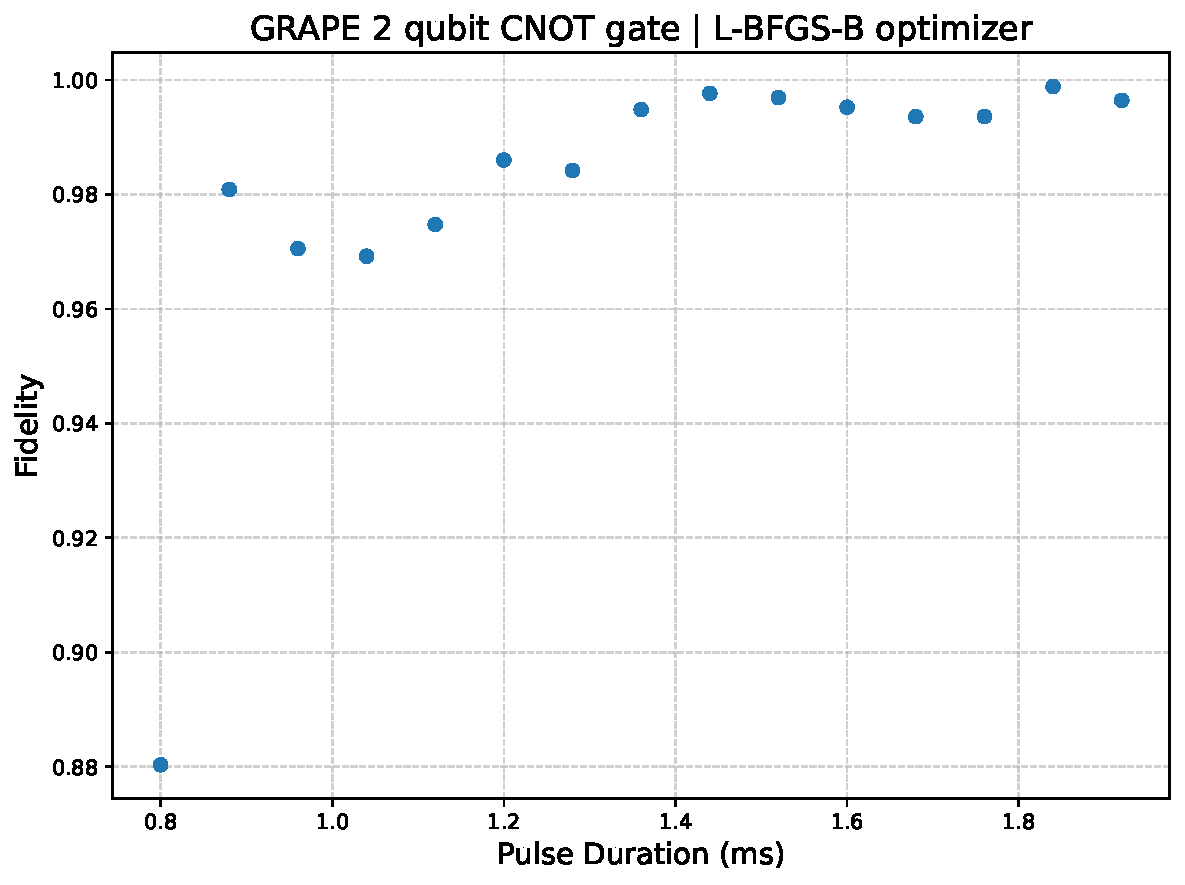
\includegraphics[width=0.8\textwidth]{images/grape_cnot_fidelity.pdf}
    \caption{GRAPE-implemented CNOT gate theoretical fidelity for different pulse durations. Each data point represents the best theoretical fidelity obtained for a given pulse duration.}
    \label{fig:grape_cnot_tstudy}
\end{figure}

The selected pulse of duration 1.04~ms achieved an experimental fidelity of 87.13\%, and its pulse profile is shown in Figure~\ref{fig:cnot_tstudy3}. Although the CNOT gate represents only a portion of the complete desired operation, this considerable increase in experimental fidelity is promising for the subsequent optimization of the complete destructive SWAP test operation. As it is a more complex optimization problem, this pulse sequence should provide a more accurate initial guess for the optimizer to refine.

\begin{figure}[ht]
    \centering
    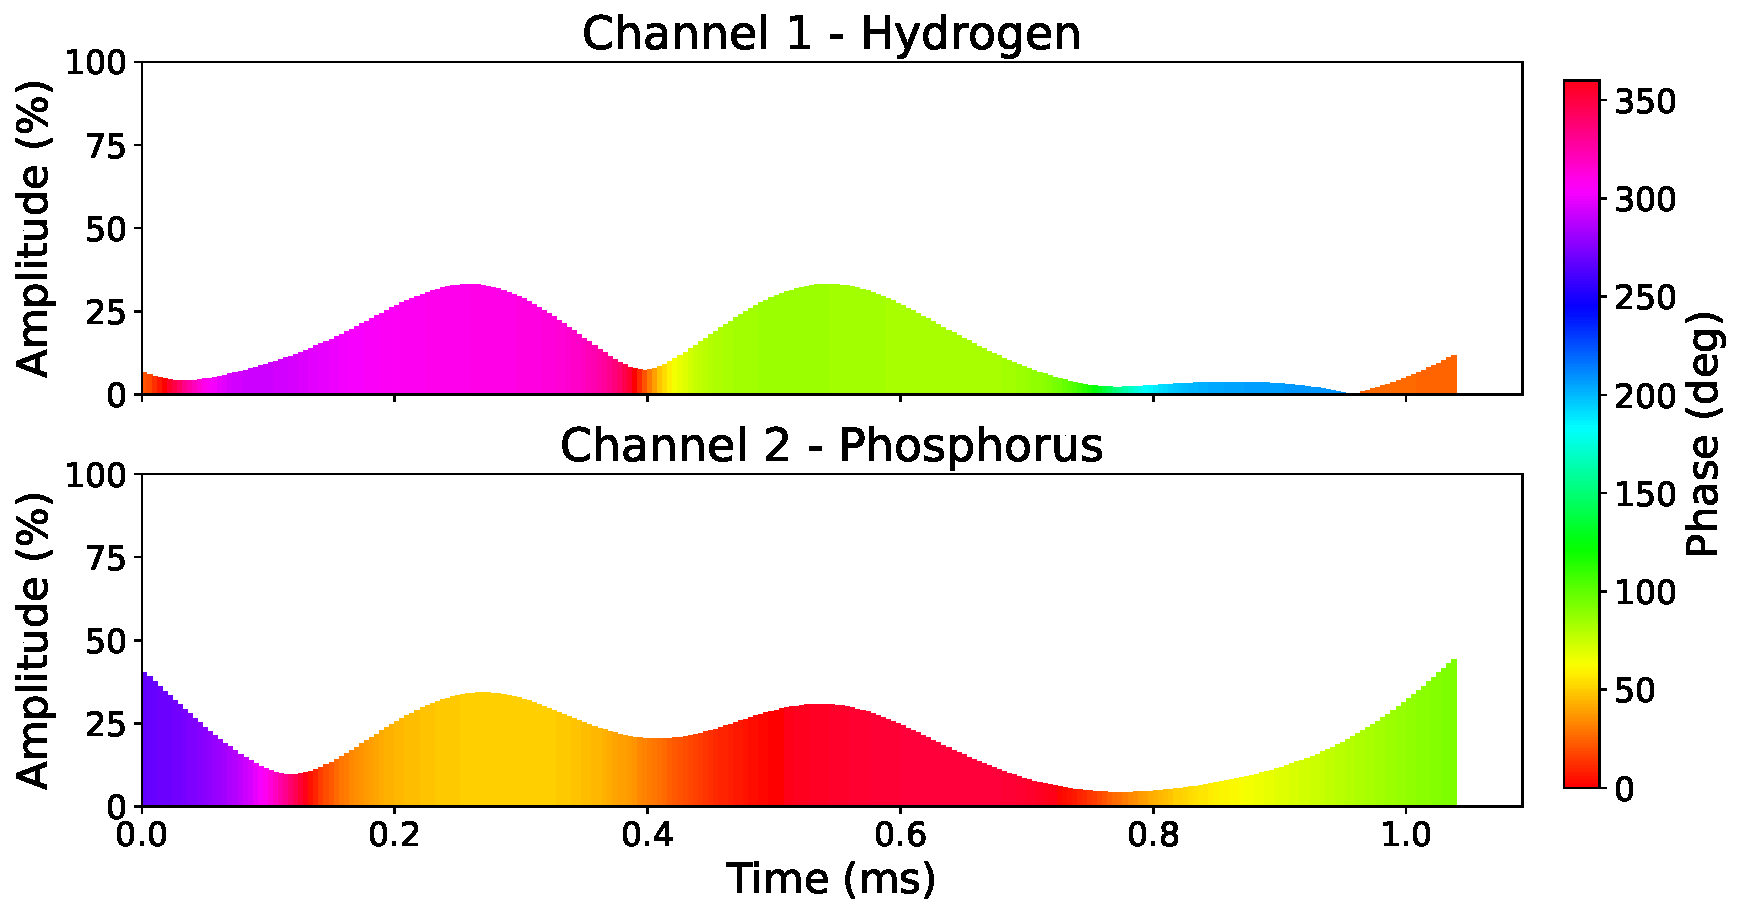
\includegraphics[width=0.8\textwidth]{images/cnot_tstudy3.pdf}
    \caption{Pulse profile for the CNOT test optimization with a duration of 1.04~ms. Experimental fidelity of 87.13\%. This pulse sequence was used as a portion of the initial guess for the composite pulse optimization of the complete destructive SWAP test operation.}
    \label{fig:cnot_tstudy3}
\end{figure}

As discussed in Section~\ref{subsec:single_qubit_operations}, single-qubit rotations can be implemented accurately using hard pulses. Accordingly, the Hadamard gate, which is equivalent to a sequence of single-qubit rotations, was implemented as a hard-pulse \(\pi/2\) rotation about the \(\hat{x}\) axis followed by a \(\pi\) rotation about the \(\hat{z}\) axis, and appended to the optimized CNOT pulse to form the initial guess for the composite pulse optimization of the complete destructive SWAP test operation.

The optimized composite pulse achieved a theoretical fidelity of 97.46\% before convergence and an experimental fidelity of 89.66\%, representing a substantial improvement over the direct optimization approach.

\begin{figure}[ht]
    \centering
    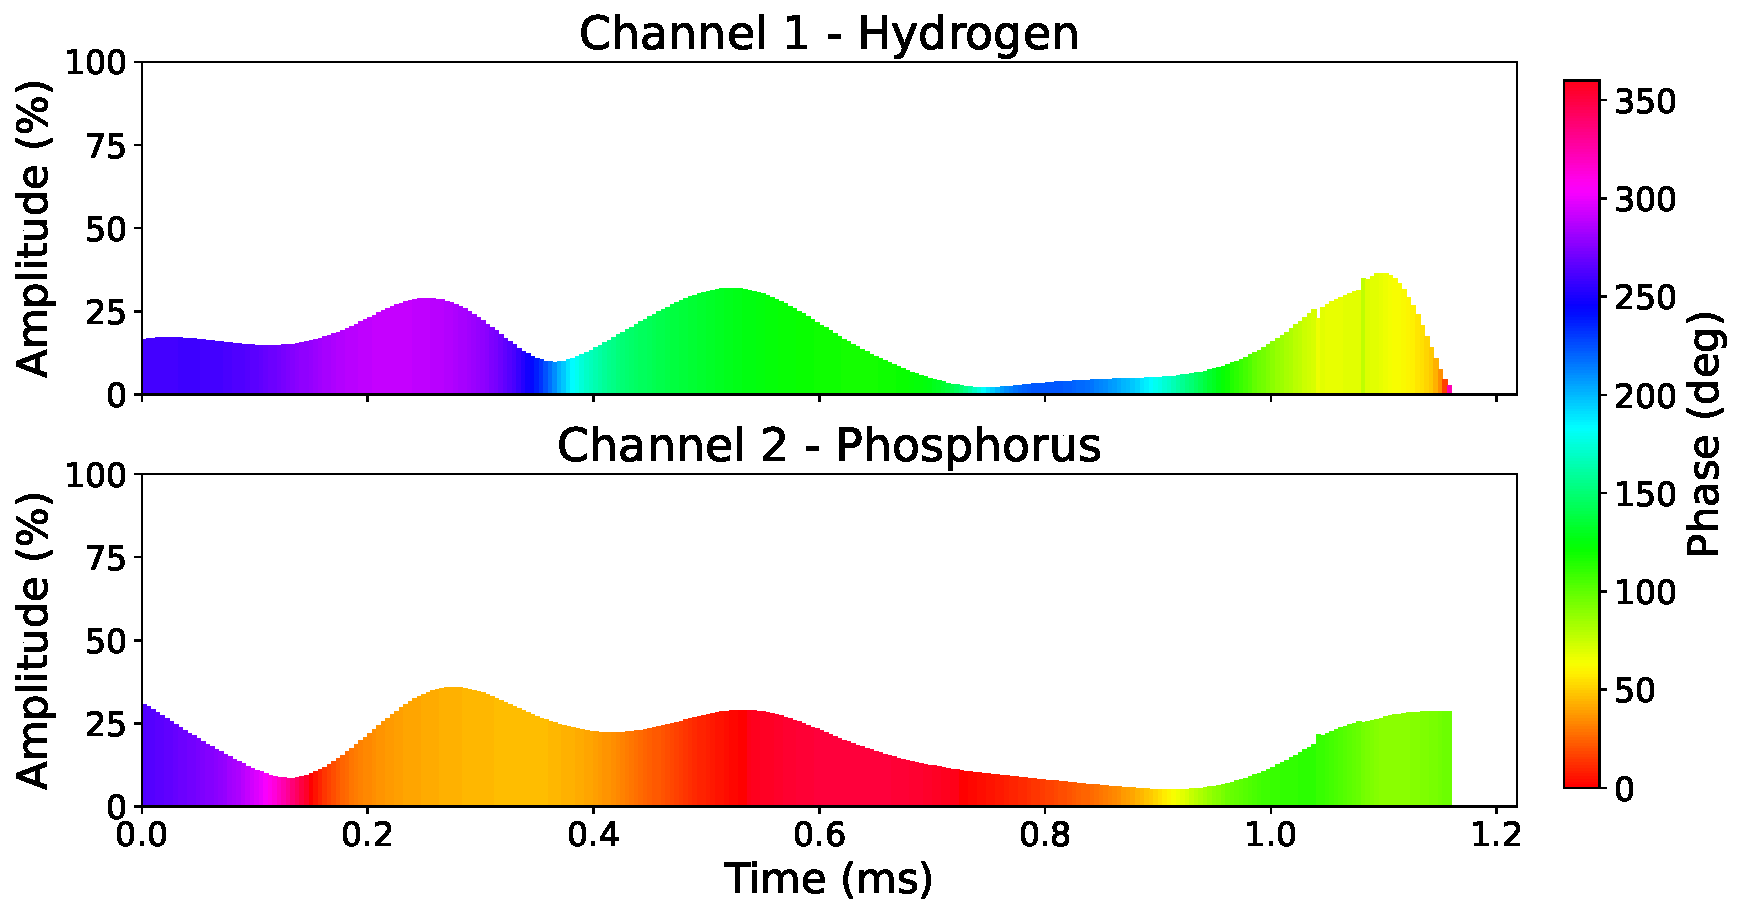
\includegraphics[width=0.8\textwidth]{images/swap_test_composite.pdf}
    \caption{Pulse profile for the destructive SWAP test optimization with a composite initial guess. Experimental fidelity of 89.66\%.}
    \label{fig:swap_composite}
\end{figure}

\subsection{Gate characterization}
\label{subsec:gate_characterization}

%In this section, the figures are the experimental density matrix results from the NMR QC.

Finally, to further characterize the performance of the destructive SWAP test control pulse, it was applied to multiple pairs of input states selected from the set \(\{|0\rangle, |1\rangle, |+\rangle, |-\rangle\}\). For each input pair, the probability of measuring the outcome \(|11\rangle\) was extracted, from which the overlap between the input states was calculated using:

\begin{equation}
    |\langle\psi|\phi\rangle|^2 = 1 - 2P(|11\rangle)
\end{equation}

The experimentally determined overlaps were then compared with their corresponding theoretical values. The experimental results reveal multiple distinct behaviors depending on the choice of input states. For example, when comparing identical states such as \(|+\rangle\) and \(|+\rangle\), or \(|-\rangle\) and \(|-\rangle\), the calculated overlaps are very close to the expected value of 1. In these cases, the small observed probability of measuring the state \(|11\rangle\) can be attributed to thermal noise and other experimental imperfections, such as decoherence.

% Figure: plus_plus
% Figure: minus_minus

For orthogonal states such as \(|+\rangle\) and \(|-\rangle\), the measured probability of the \(|11\rangle\) outcome slightly exceeded the expected value of 0.5, regardless of which state was assigned to the control qubit, as shown in Figures~\ref{fig:plusminus} and~\ref{fig:minusplus}. On the other hand, for the state pair \(|0\rangle\) and \(|1\rangle\), the measured probability of \(|11\rangle\) was consistently lower than expected. This discrepancy was more apparent when the control qubit was prepared in the state \(|1\rangle\), for which the measured probability was approximately half the expected value. This is illustrated in Figures~\ref{fig:zeroone} and~\ref{fig:onezero}.

\begin{figure}[ht]
    \centering
    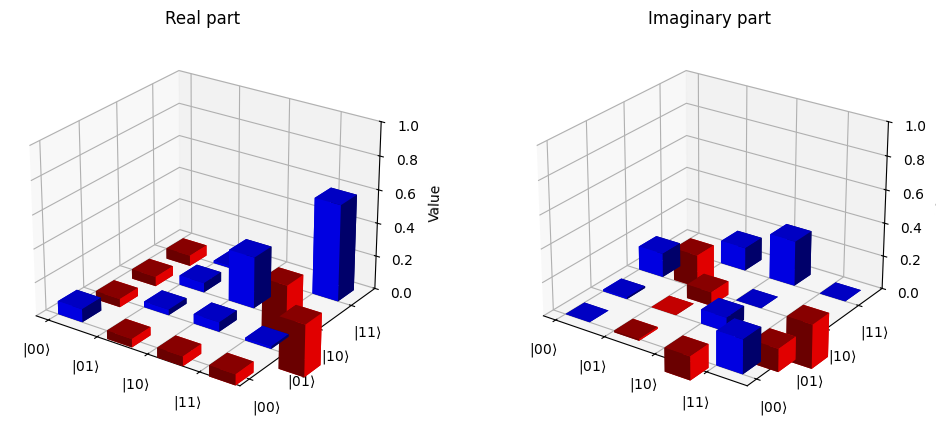
\includegraphics[width=0.8\textwidth]{images/plusminus.png}
    \caption{Experimental density matrix for the input state pair \(|+\rangle\) and \(|-\rangle\).}
    \label{fig:plusminus}
\end{figure}

\begin{figure}[ht]
    \centering
    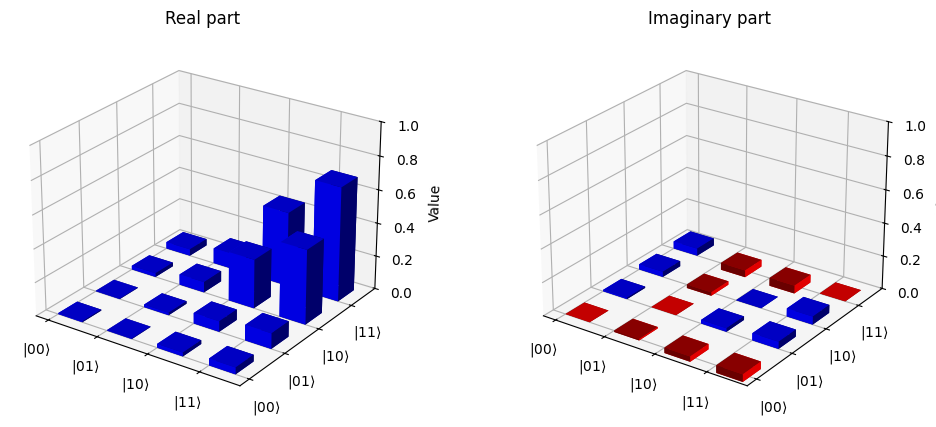
\includegraphics[width=0.8\textwidth]{images/minusplus.png}
    \caption{Experimental density matrix for the input state pair \(|-\rangle\) and \(|+\rangle\).}
    \label{fig:minusplus}
\end{figure}



\begin{figure}[ht]
    \centering
    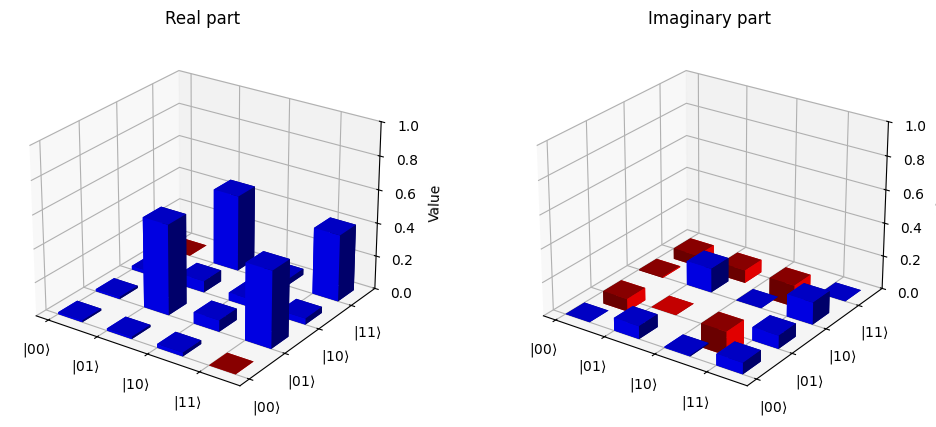
\includegraphics[width=0.8\textwidth]{images/zeroone.png}
    \caption{Experimental density matrix for the input state pair \(|0\rangle\) and \(|1\rangle\).}
    \label{fig:zeroone}
\end{figure}

\begin{figure}[ht]
    \centering
    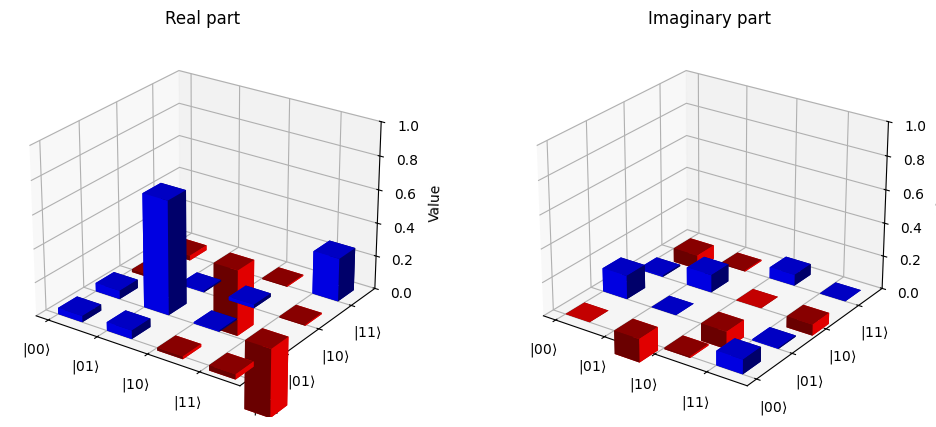
\includegraphics[width=0.8\textwidth]{images/onezero.png}
    \caption{Experimental density matrix for the input state pair \(|1\rangle\) and \(|0\rangle\).}
    \label{fig:onezero}
\end{figure}

More significantly, for some input state pairs, exchanging the roles of the control and target qubits produced substantially different results. This behavior was observed for the state pairs \(|1\rangle\) and \(|+\rangle\), and \(|0\rangle\) and \(|-\rangle\), as illustrated by the experimental density matrices in Figures~\ref{fig:minuszero} and~\ref{fig:plusone}. Since the ideal destructive SWAP test is symmetric with respect to the two input states, these results indicate that the implemented CNOT operation deviates from the ideal behavior. Consequently, further optimization of the CNOT pulse used to construct the initial guess for the composite pulse optimization is required.

\begin{figure}[ht]
    \centering
    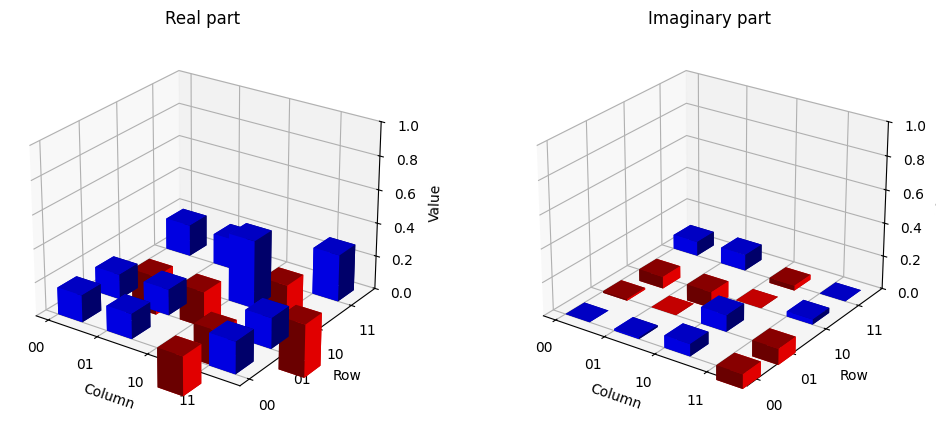
\includegraphics[width=0.8\textwidth]{images/plusone.png}
    \caption{Experimental density matrix for the input state pair \(|+\rangle\) and \(|1\rangle\).}
    \label{fig:plusone}
\end{figure}

\begin{figure}[ht]
    \centering
    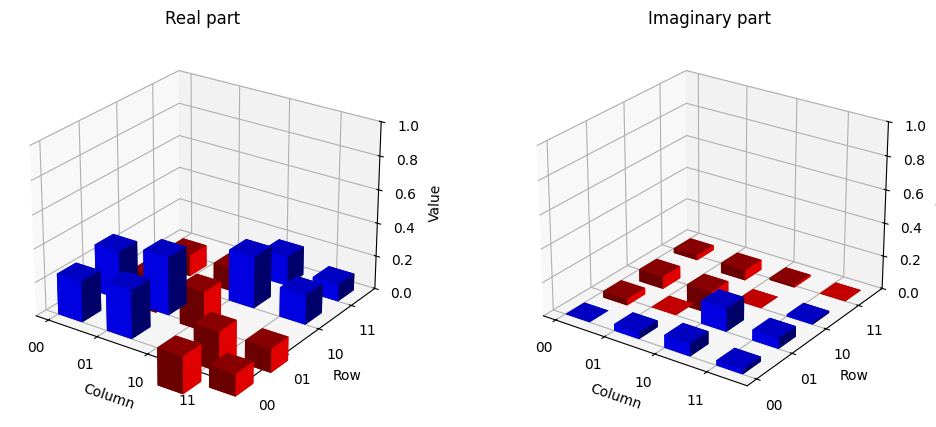
\includegraphics[width=0.8\textwidth]{images/oneplus.png}
    \caption{Experimental density matrix for the input state pair \(|1\rangle\) and \(|+\rangle\).}
    \label{fig:oneplus}
\end{figure}

\begin{figure}[ht]
    \centering
    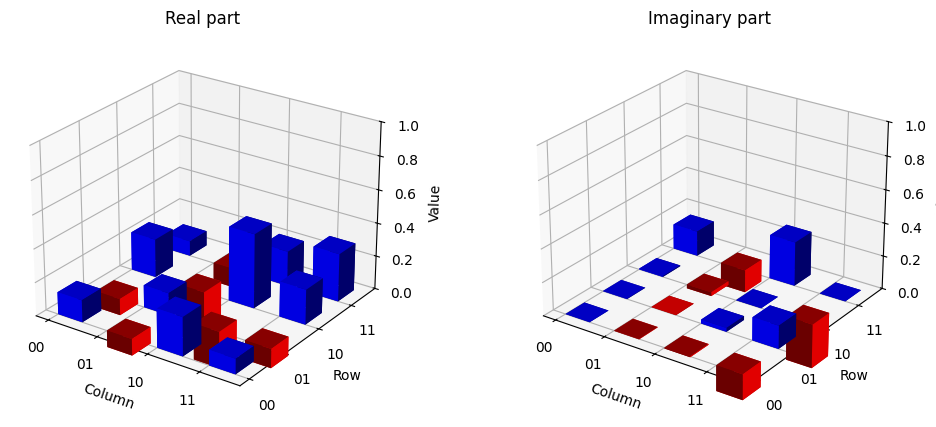
\includegraphics[width=0.8\textwidth]{images/minuszero.png}
    \caption{Experimental density matrix for the input state pair \(|-\rangle\) and \(|0\rangle\).}
    \label{fig:minuszero}
\end{figure}

\begin{figure}[ht]
    \centering
    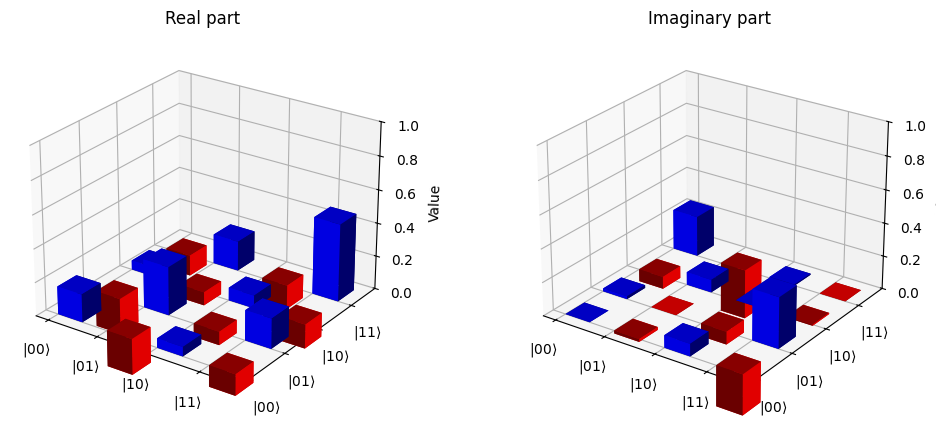
\includegraphics[width=0.8\textwidth]{images/zerominus.png}
    \caption{Experimental density matrix for the input state pair \(|0\rangle\) and \(|-\rangle\).}
    \label{fig:zerominus}
\end{figure}


